\documentclass[12pt,a4paper]{article}

\usepackage[french]{babel}
\usepackage[utf8]{inputenc}
\usepackage[T1]{fontenc}
\usepackage[top=1cm,bottom=1cm,right=1cm,left=1cm]{geometry}
\usepackage{graphicx}
\usepackage{fancyhdr}
\usepackage{hyperref}


\usepackage{amsfonts, amsmath, amssymb, amstext, latexsym}
\usepackage{epsfig}
\usepackage{exscale}
\usepackage{amsbsy}
\usepackage{amsopn}
\usepackage{listings}

\newcommand{\noi}{\noindent}
\newcommand{\dsp}{\displaystyle}
\newcommand{\ind}{{{\large 1} \hspace*{-1.6mm} {\large 1}}}


%%%%%%%%%%%%%%%%%%%%%%%%%%%%%%%   Page de garde   %%%%%%%%%%%%%%%%%%%%%%%%%%%%%%%%%%%%%%%%

% variable à redéfinir (placées sur la page de garde et sur l'entête)
\def\typedeprojet{Systèmes d'information géographiques}
\def\nomduprojet{TP OpenStreetMap}
\def\dateduprojet{Octobre 2017}

% définition des entêtes et pieds de page
\pagestyle{fancy}

% définition des marges pour les entêtes et pieds de page
\renewcommand{\headrulewidth}{0.1pt}
\renewcommand{\footrulewidth}{0.1pt}

% entête de page
\lhead{
\includegraphics[height=1.2cm]{logo_ensimag.jpg}}
\chead{\bf \typedeprojet}
\rhead{\nomduprojet}

% pied de page
\lfoot{}
\cfoot{}
\rfoot{\thepage}

% compte à partir de 0 => la 2e page est donc à 1
\setcounter{page}{0}

% re-définition des tailles d'entête et de texte
\setlength{\headheight}{60pt}
\setlength{\textheight}{710pt}

% titre de la page de garde
\title{
	% illustrations
	\begin{flushleft}
		
\includegraphics[width=5cm]{logo_ensimag.jpg} \hfill
	\end{flushleft} 
	% séparateur 1
	{\rule{15cm}{1mm}}\vspace{7mm}
	% titres
	\begin{tabular}{p{0cm} r}
		& {\Huge {\bf \typedeprojet}} \\[20pt]
		& {\huge \nomduprojet}
	\end{tabular}\\
	% séparateur 2
	\vspace{7mm}{\rule{15cm}{1mm}}\vspace{2mm} \\
	% date
	\hfill \large \dateduprojet \hspace{2cm}
	% table des matières
	\vfill
}

% auteur(s)
\author{
	\begin{tabular}{p{15cm}}
		\Large Maxime Deloche, Ludovic Carré \& Vincent Lefoulon
	\end{tabular} \\
	\hline
}

% pas de date, elle est dans le titre
\date{}

\begin{document}
\maketitle

\thispagestyle{empty} % pas de numérotation de la page de garde
\newpage

%%%%%%%%%%%%%%%%%%%%%%%%%%%%%%%%%%%%%%%%%%%%%%%%%%%%%%%%%%%%%%%%%%%%%%%%%%%%%%%%%%%%%%%%%%

\section*{Question 1}

\begin{lstlisting}[language=SQL]
SELECT COUNT(id) FROM users;
\end{lstlisting}

\begin{lstlisting}
count 
-------
  4576
  (1 row)
\end{lstlisting}

\vspace{1cm}
\section*{Question 2.a}

\begin{lstlisting}[language=SQL]
SELECT ST_X(geom), ST_Y(geom), ST_Z(geom)
FROM nodes WHERE id = 1787038609;
\end{lstlisting}

\begin{lstlisting}
st_x      |   st_y    | st_z 
----------+-----------+------
5.7680106 | 45.192893 |     
(1 row)
\end{lstlisting}

\vspace{1cm}
\section*{Question 2.b}

\begin{lstlisting}[language=SQL]
SELECT *
FROM spatial_ref_sys
WHERE srid = (
    SELECT ST_SRID(geom) FROM nodes WHERE id = 1787038609
);
\end{lstlisting}

\begin{lstlisting}
GEOGCS["WGS 84",DATUM["WGS_1984",SPHEROID["WGS 84",...
\end{lstlisting}

Le système de coordonnées utilisé est WGS84, c'est-à-dire le système GPS.

\vspace{1cm}
\section*{Question 3}

\begin{lstlisting}[language=SQL]
SELECT ST_AsEWKT(ST_Centroid(linestring)) FROM ways
WHERE tags->'amenity' = 'townhall' AND tags->'name' like '%Grenoble%';
\end{lstlisting}

\begin{lstlisting}
st_asewkt                      
----------------------------------------------------
 SRID=4326;POINT(5.73643908557793 45.1864548121024)
 (1 row)
\end{lstlisting}

La fonction ST\_AsEWKT \(Well-Known Text\) retourne une représentation textuelle d'un objet 'geometry'.

\vspace{1cm}
\section*{Question 4}

\begin{lstlisting}[language=SQL]
SELECT tags->'highway', COUNT(id) FROM ways WHERE tags?'highway'
GROUP BY tags->'highway' ORDER BY COUNT(id) DESC;
\end{lstlisting}

\begin{lstlisting}
?column?                 | count 
-------------------------+-------
residential              | 94356
unclassified             | 77678
service                  | 64461
track                    | 58276
tertiary                 | 21923
footway                  | 21742
path                     | 21413
secondary                | 18444
...
\end{lstlisting}

\vspace{1cm}
\section*{Question 5.a}

\begin{lstlisting}[language=SQL]
SELECT tags->'highway', SUM(ST_Length(linestring))
FROM ways WHERE tags?'highway'
GROUP BY tags->'highway' ORDER BY SUM(ST_Length(linestring)) DESC;
\end{lstlisting}

\begin{lstlisting}
?column?                 |         sum          
-------------------------+----------------------
unclassified             |     435.285712879273
track                    |     343.366696791793
residential              |     210.396982404606
tertiary                 |     208.294200085326
path                     |     134.367018999509
...
\end{lstlisting}

\vspace{1cm}
\section*{Question 5.b}

La \href{http://postgis.org/docs/ST_Length.html}{documentation} dit : \textit{geometry are in units of spatial reference and geography are in meters (default spheroid)}

\begin{lstlisting}[language=SQL]
SELECT * FROM spatial_ref_sys
WHERE srid = (SELECT ST_SRID(linestring) FROM ways LIMIT 1);
\end{lstlisting}

\begin{lstlisting}
GEOGCS["WGS 84",DATUM["WGS_1984",SPHEROID["WGS 84",...
\end{lstlisting}

Le système de référence est WGS84 et l'unité est donc le degré (\textit{degree}).

\vspace{1cm}
\section*{Question 5.c}

On travaille avec des géographies, dont l'unité est le mètre.

\begin{lstlisting}[language=SQL]
SELECT tags->'highway', SUM(ST_Length(linestring::geography))/1000
FROM ways WHERE tags ? 'highway'
GROUP BY tags->'highway' ORDER BY SUM(ST_Length(linestring)) DESC;
\end{lstlisting}

\begin{lstlisting}
         ?column?         |      ?column?      
--------------------------+--------------------
 unclassified             |   39840.3847465004
 track                    |   31548.5308675041
 residential              |    19217.248646164
 tertiary                 |   19092.5143218903
 path                     |   12385.5371652032
 secondary                |   11054.7544485223
 service                  |   5721.88752214514
 primary                  |   4905.59039039862
 motorway                 |   2645.76412625689
 footway                  |    2452.9424121304
 cycleway                 |   927.600411902203
 road                     |   769.272454468655
 trunk                    |   647.685572912772
 motorway_link            |   505.818144374077
...
\end{lstlisting}

\vspace{1cm}
\section*{Question 6}

On récupère tous les bâtiments de l'Ensimag depuis la table \verb?relation_members?.

\begin{lstlisting}[language=SQL]
SELECT SUM(ST_Area(ST_MakePolygon(ways.linestring)::geography))
FROM relations, relation_members, ways
WHERE
	relation_members.relation_id = relations.id AND
	relation_members.member_id = ways.id AND
	relations.tags->'name' = 'Ensimag';
\end{lstlisting}

\begin{lstlisting}
       sum
------------------
 2640.86233445186
(1 ligne)
\end{lstlisting}

\vspace{1cm}
\section*{Question 7}

On considère qu'une école est contenue dans un quartier si sa zone géographique (\textit{linestring})
est incluse dans celle du quartier. On commence par déterminer le système
géographique utilisé par la table \verb?quartier? :

\begin{lstlisting}[language=SQL]
SELECT ST_SRID(the_geom) FROM quartier;
\end{lstlisting}

\begin{lstlisting}[language=SQL]
st_srid 
---------
    2154
    2154
    2154
    2154
    2154
    2154
    2154
    2154
    2154
    2154
    2154
    2154
    2154
    2154
    2154
    2154
    2154
    2154
    2154
    2154
    2154
    2154
    2154
\end{lstlisting}

Puis on convertit les écoles en polygones et les transforme dans le bon système géographique avant de vérifier la relation d'inclusion avec les quartiers.

\begin{lstlisting}[language=SQL]
SELECT quartier.quartier, count(ways.id)
FROM quartier, ways
WHERE
    ways.tags->'amenity' = 'school' AND
    ST_Contains(
        quartier.the_geom,
        ST_Transform(ways.linestring, 2154)
    )
GROUP BY quartier.quartier ORDER BY count(ways.id) DESC;
\end{lstlisting}

\begin{lstlisting}
quartier             | count 
---------------------+-------
BERRIAT ST BRUNO     |    13
CENTRE VILLLE        |    12
EXPOSITION-BAJATIERE |     9
RONDEAU-LIBERATION   |     7
EAUX CLAIRES         |     6
ABBAYE-JOUHAUX       |     5
...
\end{lstlisting}

\vspace{1cm}
\section*{Question 8 (incomplet)}

On définit le centre géographique d'une région comme la municipalité ayant une
distance minimale avec sa municipalité la plus éloignée. On définit la distance
entre deux villes comme celle entre les centroïdes des centroïdes de leurs bâtiments.

On commence par récupérer les municipalités :

\begin{lstlisting}[language=SQL]
SELECT *
FROM relations
WHERE tags->'boundary' = 'administrative' AND tags->'admin_level' = '8';
\end{lstlisting}

Une relation contient plusieurs éléments géométriques, listés dans la table
\verb?relation_members? :

\begin{lstlisting}[language=SQL]
SELECT *
FROM relations
INNER JOIN relation_members 
ON relations.id = relation_members.relation_id
WHERE tags->'boundary' = 'administrative' 
AND tags->'admin_level' = '8';
\end{lstlisting}

\verb?relation_members.member_type? fait référence à la table contenant les données
géographiques :

\begin{lstlisting}[language=SQL]
SELECT DISTINCT(member_type)
FROM relation_members;
\end{lstlisting}

\begin{lstlisting}
member_type 
-------------
W
R
N
(3 rows)
\end{lstlisting}

Les bâtiments d'une ville sont stockés dans la table \verb?ways?. On calcule le centroïd
de chaque municipalité :

\begin{lstlisting}[language=SQL]
SELECT relations.id, ST_Centroid(ST_Union(ways.linestring))
FROM relations
JOIN relation_members ON relations.id = relation_members.relation_id
JOIN ways ON relation_members.member_id = ways.id
WHERE
    relations.tags->'boundary' = 'administrative' AND
    relations.tags->'admin_level' = '8' AND
    relation_members.member_type = 'W'
GROUP BY relations.id;
\end{lstlisting}

TODO : ce que contient la table ways pour les municipalités est étrange. Notamment,
il n'y a aucune ligne avec building=yes.

Puis, pour chaque ville, on calcule sa distance aux autres, prend celle maximale
et retourne la ville ayant la plus petite :

\begin{lstlisting}[language=SQL]
\end{lstlisting}

\vspace{1cm}
\section*{Question 9 (incomplet)}

Par "endroit", on comprendra deux choses :

\begin{itemize}
	\item Le centroïde d'un bâtiment ;
	\item Un point géographique n'appartenant pas à un bâtiment.
\end{itemize}

Dans le premier cas, notre lieu de vacances est un bâtiment éloigné d'au moins
10 kilomètres de tout autre bâtiment. Pour les trouver, on peut simplement
calculer les distances deux à deux entre les centroïdes des bâtiments.

Dans le deuxième cas, notre lieu de vacances n'est pas un bâtiment. Être éloigné
de 10 kilomètres de toute autre structure signifie alors que ces bâtiments sont
eux-mêmes éloignés d'au moins 2*10 kilomètres.

\begin{lstlisting}
   > 10km        > 10km
B -------- * ------------- B
\end{lstlisting}

\vspace{1cm}
\section*{Documentation de l'implémentation Java}

\subsection*{Usage}

Un Makefile permet d'utiliser le projet. 
\begin{itemize}
	\item \verb?make? : compile le projet
    \item \verb?make run? : compile et lance le projet. Par défaut, tout est tracé. On peut en revanche ne tracer que certains éléments en les ajoutant à la suite de \verb?make run? :
		\begin{itemize}
				\item \verb?buildings? : affiche les immeubles
				\item \verb?roads? : affiche les routes
				\item \verb?noise? : affiche les zones de pollution sonore
				\item \verb?stations? : affiche les stations de transport
				\item \verb?schools? : affiche le nombre d'écoles par quartier
				\item \verb?densities? : affiche la densité
		\end{itemize}
		Par exemple : \verb?make run buildings roads stations?.

    \item \verb?make Question10? : compile et lance le code de la question 10 (test de l'accès à la base de données)
    \item \verb?make Question11? : compile et lance le code de la question 11 (points dont le nom ressemble à "Dom\_\_ne \_niversit\%"
\end{itemize}

\subsection{Bonus}

Les questions bonus 14\_a et 14\_b ont été implémentées. La question A récupère les noms et centroïdes de chacun des quartiers ainsi que le nombre d'écoles dans ces derniers. Le package graphique ne permet pas d'afficher du texte à l'écran (ce que l'on aurait pu faire avec un JLabel par exemple) et on a donc choisi d'utiliser un code pour représenter le nombre d'écoles dans un quartier.

Un cercle de couleur est donc ajouté au centroïde de chacun de ces quartiers, la correspondance couleur/nombre d'écoles est donné par le programme lors de son exécution.
L'intérêt de la question étant la requête avec les bonnes coordonnées géographiques pour l'affichage, nous n'avons pas réimplémenté JLabel ou écrit du code compliqué pour le choix de la couleur d'un point.

Cela implique que le code ne peut pas être exécuté sur une autre ville que Grenoble puisque l'association couleur/écoles est fixe et propre à Grenoble.

Pour la question 14\_b, nous avons représenté la nuisance sonore par des polygones. La taille de la zone considérée comme affectée par la nuisance a été fixée, après une rapide recherche, à 200m des sources de nuisance. Une fonction plus précise nécessiterait d'évaluer la puissance des nuisances et leur degré d'atténuation en fonction de la distance.

\subsection*{Architecture du code}

Le code se base sur une architecture basique MVC :

\begin{itemize}
\item Il n'y a qu'un seul contrôleur, le fichier \verb?Main.java?
\item Le package \verb?models? contient les classes effectuant les requêtes à la base de données \item Les classes du package \verb?views? se chargent de l'affichage graphique
\end{itemize}

TODO : choix de conception particuliers ?

\subsection*{Requêtes SQL}

Les requêtes SQL sont effectuées via la classe statique \verb?models.DataBase?. Elle s'occupe de sauvegarder un objet Connection, et contient les fonctions :
\begin{itemize}
	\item \verb?getQuartierSchool()? : retourne la liste des quartiers (\verb?Quartier?)
	\item \verb?getBuildingWays()? : retourne la liste des immeubles (\verb?Polygon?)
	\item \verb?getRoadWays()? : retourne la liste des routes (\verb?LineString?)
    \item \verb?getBoundaries()? : retourne la liste des frontières entre quartiers (\verb?LineString?)
    \item \verb?getNoisePollutedZones()? : retourne la listes des zones (\verb?Polygon?) soumises à des nuisances sonores
\end{itemize}

Les requêtes récupèrent des objets org.postgis et les convertissent (via des fonctions privées) en objets (Polygon, LineString...) de notre modèle.

Toutes ces requêtes sont effectuées sur la ville de Grenoble : une variable globale en début de fichier est à ajouter à la clause WHERE des requêtes, ce qui permet de changer facilement les coordonnées de la zone couverte par l'application.

\subsubsection*{Question 12}

\begin{lstlisting}[language=SQL]
SELECT ST_Transform(linestring, 2154) FROM ways
WHERE ST_XMin(bbox) > 5.7 AND ST_XMax(bbox) < 5.8
AND ST_YMin(bbox) > 45.1 AND ST_YMax(bbox) < 45.2
AND tags?'building';
\end{lstlisting}

Cette requête nous donne tous les bâtiments dans Grenoble avec la projection Lambert. Ces géométries sont ensuite converties en Polygones par l'application Java.

\begin{lstlisting}[language=SQL]
SELECT ST_Transform(linestring, 2154) FROM ways
WHERE ST_XMin(bbox) > 5.7 AND ST_XMax(bbox) < 5.8
AND ST_YMin(bbox) > 45.1 AND ST_YMax(bbox) < 45.2
AND tags?'highway';
\end{lstlisting}

Cette requête nous donne tous les routes dans Grenoble avec la projection Lambert. Ces géométries sont ensuite converties en Linestring par l'application Java.

\subsubsection*{Question bonus 13}

\begin{lstlisting}[language=SQL]
SELECT ST_Transform(geom, 2154) FROM nodes
WHERE ST_X(geom) BETWEEN 5.7 AND 5.8
AND ST_Y(geom) BETWEEN 45.1 AND 45.2
AND tags?'public_transport';
\end{lstlisting}

Cette requête nous donne tous les arrêts de transport public de Grenoble. Ces géométries sont ensuite converties en Point par l'application Java.

\subsubsection*{Question bonus 14\_a}

\begin{lstlisting}[language=SQL]
SELECT quartier.quartier, ST_X(ST_Centroid(quartier.the_geom)) AS X, 
ST_Y(ST_Centroid(quartier.the_geom)) AS Y, COUNT(ways.id) 
FROM quartier, ways
WHERE ways.tags->'amenity' = 'school'
AND ST_Contains(quartier.the_geom, ST_Transform(ways.linestring, 2154))
GROUP BY quartier.quartier, X, Y;
\end{lstlisting}

La requête est pratiquement identique à celle de la question 7, on compte le nombre d'écoles contenu par quartier et l'on récupère le nom et la longitude/latitude du centroïde de chacun des quartiers.
La question parle de boulangeries en faisant référence à la question 7, mais la question parle d'écoles donc j'ai supposé qu'il s'agissait d'une erreur dans l'énoncé.


\subsubsection*{Question bonus 14\_b}

\begin{lstlisting}[language=SQL]
SELECT ST_Buffer(ST_Transform(linestring, 2154), 200) FROM ways
WHERE ST_XMin(bbox) > 5.7 AND ST_XMax(bbox) < 5.8
AND ST_YMin(bbox) > 45.1 AND ST_YMax(bbox) < 45.2
AND (tags->'aeroway' = 'areodrome'
	OR tags->'highway' = 'motorway' OR tags->'railway' = 'rail'
);
\end{lstlisting}

Cette requête nous donne toutes les voies de type aéroport, chemin de fer ou autoroute de Grenoble. Ces géométries sont ensuite converties en Polygones par l'application Java.

\subsubsection*{Question bonus 14\_c}

Pour simplifier le quadrillage, on considère la région Rhône-Alpes comme rectangulaire.
On commence par récupérer ses coins :

\begin{lstlisting}[language=SQL]
SELECT MAX(ST_XMax(linestring)) as xmax,
       MAX(ST_YMax(linestring)) as ymax,
       MIN(ST_XMin(linestring)) as xmin,
       MIN(ST_YMin(linestring)) as ymin
FROM ways;
\end{lstlisting}

On génère ensuite le quadrillage avec la fonction SQL fournie \href{https://gis.stackexchange.com/a/16390}{ici}.
Pour cela, on récupère les dimensions du rectangle et détermine les paramètres
de la grille :

\begin{lstlisting}
dy = ymax - ymin = 4.216852
dx = xmax - xmin = 7.2422614
xsize = 0.2 (Il faut que dx en soit multiple. On arrondit dx a 7.2)
ysize = 0.2 (Il faut que dy en soit multiple. On arrondit dy a 4.2)
nrow = 4.2 / 0.2 = 21
ncol = 7.2 / 0.2 = 36
x0 = xmin
y0 = ymin
\end{lstlisting}

On peut alors générer le quadrillage :

\begin{lstlisting}[language=SQL]
SELECT * FROM ST_CreateFishnet(36, 21, 0.2, 0.2, 0.6986247, 43.3160588);
\end{lstlisting}

\begin{lstlisting}
row | col |                                                                                            geom                                                                                            
-----+-----+--------------------------------------------------------------------------------------------------------------------------------------------------------------------------------------------
1 |   1 | 01030000000100000005000000A1B0D52F225BE63F77CE609D74A84540A1B0D52F225BE63F1168FA360EC2454008173C9688C1EC3F1168FA360EC2454008173C9688C1EC3F77CE609D74A84540A1B0D52F225BE63F77CE609D74A84540
2 |   1 | 01030000000100000005000000A1B0D52F225BE63F1168FA360EC24540A1B0D52F225BE63FAB0194D0A7DB454008173C9688C1EC3FAB0194D0A7DB454008173C9688C1EC3F1168FA360EC24540A1B0D52F225BE63F1168FA360EC24540
3 |   1 | 01030000000100000005000000A1B0D52F225BE63FAA0194D0A7DB4540A1B0D52F225BE63F449B2D6A41F5454008173C9688C1EC3F449B2D6A41F5454008173C9688C1EC3FAA0194D0A7DB4540A1B0D52F225BE63FAA0194D0A7DB4540
...
\end{lstlisting}

La colonne \verb?geom? contient une géométrie de type polygône. Il ne reste plus,
pour chaque zone, qu'à faire l'intersection avec chaque bâtiment et regarder si
elle est nulle ou non. Contrairement à la question 7 où on testait l'inclusion,
on s'intéresse ici à l'intersection, sinon un bâtiment chevauchant plusieurs
zones ne compterait pour aucune.

Seulement, le calcul d'intersection pour toutes les zones et tous les bâtiments
est extrêmement cher donc on considérera qu'un bâtiment appartient à une
zone si son centroïde y est inclus.

Par exemple, en prenant uniquement quatre zones :

\begin{lstlisting}[language=SQL]
SELECT ST_AsText(grid.geom), COUNT(ways)
FROM ST_CreateFishnet(2, 2, 3.6, 2.1, 0.6986247, 43.3160588) as grid, ways
WHERE ST_Contains(ST_SetSRID(grid.geom, 4326), ST_Centroid(ways.linestring))
GROUP BY grid.geom;
\end{lstlisting}

\begin{lstlisting}
st_astext                   |  count  
---------------------------|----------
POLYGON((                   |   51262
    0.6986247 43.3160588,
    0.6986247 45.4160588,
    4.2986247 45.4160588,
    4.2986247 43.3160588,
    0.6986247 43.3160588
))
POLYGON((                   |  146166
    0.6986247 45.4160588,
    0.6986247 47.5160588,
    4.2986247 47.5160588,
    4.2986247 45.4160588,
    0.6986247 45.4160588
))
POLYGON((                   | 1192611
    4.2986247 43.3160588,
    4.2986247 45.4160588,
    7.8986247 45.4160588,
    7.8986247 43.3160588,
    4.2986247 43.3160588
))
POLYGON((                   | 2622439
    4.2986247 45.4160588,
    4.2986247 47.5160588,
    7.8986247 47.5160588,
    7.8986247 45.4160588,
    4.2986247 45.4160588
))
(4 rows)
\end{lstlisting}

On vérifie :

\begin{lstlisting}[language=SQL]
SELECT COUNT(ways) FROM ways;
\end{lstlisting}

\begin{lstlisting}
count  
---------
4012478
\end{lstlisting}

Or $51262 + 146166 + 1192611 + 2622439 - 4012478 = 0$. Tous les bâtiments ont
bien été associés à une zone.

\subsubsection*{Question bonus 14\_d}

Commençons par nous donner une idée des types de bâtiments à notre disposition :

\begin{lstlisting}[language=SQL]
SELECT DISTINCT(tags->'amenity') FROM ways WHERE tags ? 'amenity';
\end{lstlisting}

On choisira de représenter les zones touristiques par la densité des types de
bâtiments suivants :

\begin{lstlisting}
cinema
bar;nightclub
bar;restaurant
bar
ice_cream
nightclub
casino
pub
park
restaurant
cafe
\end{lstlisting}

On aurait aussi pu représenter les zones culturelles :

\begin{lstlisting}
school
library
theatre
college
arts_centre
conference_centre
university
\end{lstlisting}

Puis on suit la même stratégie de quadrillage qu'en 14.c.

\subsection*{Tests}

Nous avons comparé les résultats de l'affichage avec la carte de Grenoble sur le site web de openstreetmap pour vérifier la correspondance. Nous avons également confirmer le résultat sur la somme de la taille des routes de Grenoble sur Internet car la valeur ne nous semblait pas évidente.

\newpage
Voici la carte obtenue avec notre programme :

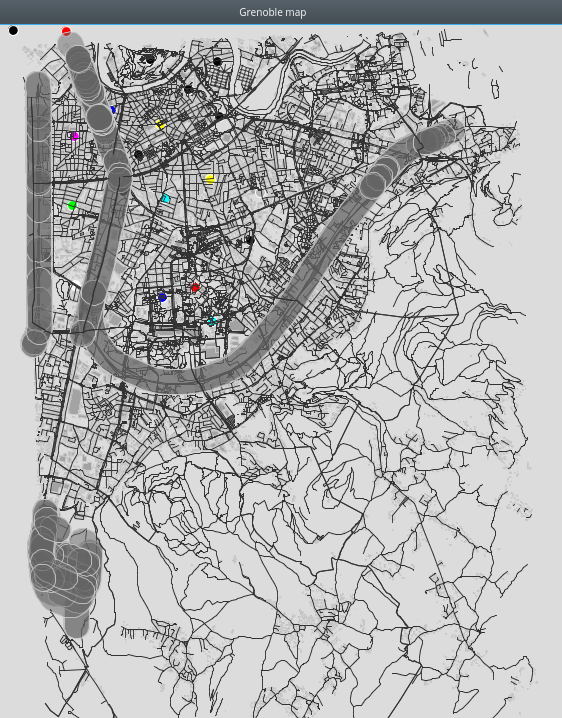
\includegraphics[height=23cm]{map.png}

\end{document}
